\documentclass{jsarticle}

\usepackage{otf}
\usepackage[dvipdfmx]{graphicx}     % png 形式を利用するために付加

\begin{document}

\tableofcontents
\newpage
\listoftables
\newpage
\listoffigures
\newpage

\section{はじめに}

近年,我が国においては,若者の旅行離れが進んでおり,地域経済・文化の発展への悪影響が懸念されている.そこで我々は,旅行を促進する観光推薦システムを通じて若者と地域を結びつける仕組みの形成し,地域活性化へ寄与することを目指した.

本章では,本研究で対象とする観光の歴史と現状についてまとめ,今後の観光の発展に向けた課題について述べる.

\newpage

\subsection{観光促進の意義}

2013年,日本政府の閣僚によって構成される観光立国推進閣僚会議が立ち上げられた.本会議で決定された「観光立国実現に向けたアクション・プログラム2014\cite{action_program_2014}では観光について次のように述べている.

\begin{quote}
観光は、急速な成長を遂げるアジアをはじめとする世界の需要を取り込むことによって、日本の力強い経済を取り戻すための柱である。加えて、人口減少・少子高齢化が進展する中、国内外からの交流人口の拡大によって地域の活力を維持し、社会を発展させるとともに、諸外国との双方向の交流により、国際相互理解を深め、国際社会での日本の地位を確固たるものとするためにも、極めて重要な分野である。
\end{quote}

また,東日本大震災からの復興を新しい国づくりの契機にしたいとして2011年に発足した有識者らによる政策発信組織である日本創世会議においても,「地方元気戦略」のひとつに観光をキーワードとして挙げており,地方へ人を呼び込む魅力づくりの施策として期待されている.

さらに,経済面から観光を調査すると,世界全体GDPに占める観光関連業界のGDPは 9.1\% であり,金融業に次いで世界第2位の業種であることがわかる.
国内においても,その経済効果は大きい.我が国の観光統計の概要を図\ref{tourism_kibo}に示す.

\begin{figure}[h!]
\begin{center}
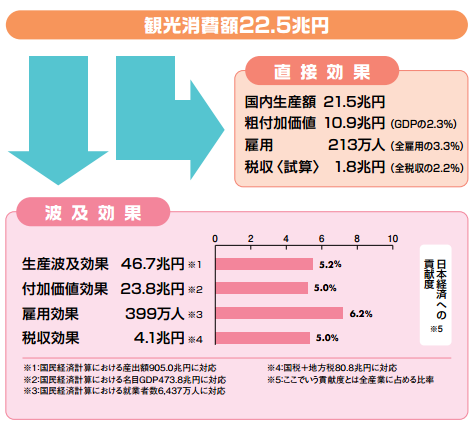
\includegraphics[width=8.0cm]{./image/tourism_kibo.png}
\caption{日本における観光統計の概要\cite{tourism_stat}}
\label{tourism_kibo}
\end{center}
\end{figure}

また,観光ビジネス研究会所属の中小企業診断士らによると,観光産業の発展を目指す理由を次のように挙げている\cite{tourism_future}.

\begin{enumerate}
\item 少子高齢化社会への対応: 国内需要の縮小が想定されるなか,我が国の伝統・文化・産業などのソフトパワーによる経済成長ができる可能性を持っている.
\item 地域経済の活性化: 地域独自の文化を含む観光資源の活用することで,国内外の旅行者との交流人口を増加させ,魅力的な地域を形成できる可能性を持っている.
\item 為替変動への対応: 観光産業は,原材料を必要としないため,安定的な経済社会の実現に向けた可能性を持っている.
\item 雇用の拡大: 若年層から熟年層まで幅広く雇用を生む可能性を持っている.
\end{enumerate}


以上のように,観光は国家戦略,経済戦略として重要な位置づけとされており,国内のみならず世界の地域文化・経済を支える分野である.したがって,観光促進に関する研究をする意義は大きい.

\subsection{観光分野の課題}

観光分野の発展はその波及効果も含めて大きな期待がされている.一方で,発展に向けた課題は数多くある.
観光行政を担当している観光庁が毎年発表している観光白書では,2010年から若者旅行の促進を課題のひとつとして毎年挙げている\cite{kanko_hakusho_2009}\cite{kanko_hakusho_2010}\cite{kanko_hakusho_2011}\cite{kanko_hakusho_2012}\cite{kanko_hakusho_2013}\cite{kanko_hakusho_2014}.観光白書では,若者の旅行離れが将来的な観光発展に大きな影響を与えることが危惧されている.この課題の解決に向けた有識者会議として2011年に若者旅行振興研究会が発足した.
本研究会では,発足にあたり次の課題を挙げている\cite{wakamono_shinko}.

\begin{enumerate}
\item 国内観光市場の低迷: 2005年以降,横ばいで推移しており,国内観光市場が発展していない
\item 日本人旅行の回数・宿泊数が減少傾向: 実質的に国内観光市場を支えている日本人旅行が低調.訪日外国人旅行は今後期待されているが,まだ市場は小さい.
\item 若者の旅行回数の減少: 20代・30代の旅行回数の落ち込みが顕著.他世代と比較して学生旅行の回数も大きく減少している.
\item 将来的に家族旅行の回数減少の懸念: 旅行回数の少ない若者がライフステージが変わったときに旅行行動をとらない可能性が高い.
\end{enumerate}

\subsection{情報推薦技術の発展}

一方,情報推薦技術の発展が近年著しい.政府においても〜

\subsection{本研究の目的}

これまでの説明によって,観光は我が国のみならず世界全体として主要な産業のひとつであり,我が国の成長にとっても重要な分野であることが明らかになった.観光庁は,観光分野の発展に向けて,若者旅行の促進を政策のひとつとあげており,若者旅行振興研究会を発足させた.本研究会では, 若者旅行振興のための課題を示している.

一方,情報工学分野においては新しい情報発信の仕組みとして情報推薦技術の実践利用が進んでいる.我々は,観光領域に情報推薦の仕組みを適用し,消費者の行動データをもとにしたパーソナライズした地域情報発信を行い,行動データの観光推薦への活用可能性を検証することを目的として研究を進めることとした.本研究によって, 観光分野の発展および地域活性化に寄与することを狙う.

\subsection{本論文の構成}

本論文は,n章から構成される.
第2章では,本研究で扱う観光の概観について調査した内容を述べる.
第3章では,情報推薦技術の概観と観光領域での活用事例について調査し,本研究で解決を目指す具体的な課題を明らかにする.
第4章では,課題解決を図った観光推薦システムの提案・設計を示す.
第5章では,開発したプロトタイプシステムの運用結果とその評価を質的観点と量的観点からまとめ,考察する.
第6章では,本研究のまとめと今後の課題について述べる.

\subsection{まとめ}

本章では,観光分野の研究を実施する意義を明らかにし,本研究の目的を,行動データの観光推薦への活用可能性の検証であることを示した.
次章以降では,既存研究,関連事例などを細かに調査し,その解決を図る.

\section{観光の概観}


\subsection{観光の歴史}

観光という言葉は,中国の「益経」という書物のなかの「国の光を観る.用て王の賓たるに利し」という一節によるとされている.\cite{kanko_define}
ここでいう「国の光」とは,国王の人徳と善政によって国が反映し,その国を訪れる人々にはその国が光に輝いて見えることをいう.すなわち,観光とは,その「国の光」を観ることである.

\subsection{観光研究の歴史}

一般に,観光は余暇の時間に実施する人間の行為であり,観光を実施するには金銭的な支出が必要であるとされている.我が国においての観光は,経済的に豊かになった高度経済成長期から盛んに注目され,これまで一部の富裕層にのみが実施できた観光が多くの国民にとって身近なものになった.
それに伴い,観光の学問的な取り組みのニーズが高まり,我が国では1960年に日本観光学会が設立され,観光研究が始まった.日本国内の主な学会を 表\ref{japanese_society} に示す.


\begin{table}[!h]
\small
\caption{日本国内の主な学会\cite{japanese_society_list}}
\begin{center}
\begin{tabular}{lll}
\label{japanese_society}
学会名 & 設立年 & 活動目的 \\ \hline
日本観光学会                            & 1960年 & 観光及び観光事業に関する学術の進歩・普及 \\
日本ホスピタリティ・マネジメント学会    & 1992年 & ホスピタリティの考え方を基軸としたマネジメント研究 \\
日本国際観光学会                        & 1993年 & 国際観光の学術研究の推進 \\
余暇ツーリズム学会                      & 2001年 & 余暇領域の研究 \\
総合観光学会                            & 2001年 & 専門分野を超えた総合観光学の確立と観光地域の持続的な発展 \\
観光まちづくり学会                      & 2001年 & 観光をまちづくりの視点で研究 \\
日本観光ホスピタリティ教育学会          & 2002年 & 観光とホスピタリティに関わる教育の在り方を探究する \\
観光情報学会                            & 2003年 & 観光学と情報科学技術に関する学術的視点と観光産業の融合 \\
長崎国際大学 国際観光学会               & 2005年 & 長崎国際大学での研究成果を公開し広く情報交換を得ること \\
日豪ツーリズム学会                      & 2007年 & 日豪観光分野における交流の促進に関して調査・研究 \\
国際観光医療学会                        & 2010年 & 観光と医療に携わる領域の研究ならびに交流 \\
日中国際ツーリズム学会                  & 2010年 & 中日ツーリズムの国際協力に関する研究 \\
コンテンツツーリズム学会                & 2011年 & コンテンツを活用した観光振興及び地域活性化の研究と実践 \\
観光学術学会                            & 2012年 & 観光学の学術的発展と普及 \\
\end{tabular}
\end{center}
\end{table}


\subsection{観光の定義}

観光学は,いまだ発展途上の学問であり,現時点で「観光」の普遍的な定義を示すのは難しいとされている\cite{kanko_define}.
観光の定義には,代表的なものがいくつかあるが,研究の必要により研究者によっては独自の定義を用いる場合も多い.

ここでは代表的な定義を示したうえで,本研究での定義を述べる.


\subsubsection{経済学としての観光定義}

観光は,経済学者が「見えざる輸出」(invisible export) として重要性に注目したことによって始まったとされている.最初の研究課題は,その経済効果をどのように測定するかである.オギルヴィエは,観光の本質が「一時的滞在地において他所で取得した収入を消費すること」と定義した.一方,グリュックスマンは,「ある土地における一時的滞在者とその土地の住民との間の諸般の関係」と考えた.

\subsubsection{一般的な定義としての観光}

特定の研究目的を念頭におかず,一般的な定義として代表的に利用されたのは,井上による「人が日常生活圏を離れて,再び戻る予定で,レクリエーションを求めて移動すること」である.

\subsubsection{我が国における公的な定義}

「余暇時間の中で,日常生活圏を離れて行う様々な活動であって,触れあい,学び,遊ぶということを目的とするもの」である.この概念をまとめたものを図\ref{define_kanko_by_unnyu} に示す.近年では,この定義を用いて観光を論ずる場合が多い.

\subsubsection{国際的な定義}

世界観光機構(WTO: World Tourism Organization) では,「訪問の主要な目的が,訪問国内で報酬を得るための活動を行うこと以外の者で,1泊以上12ヶ月を超えない期間,居住国以外の国で通常の生活環境を離れて旅行する人」としている.

\subsubsection{国際的な定義}


\subsubsection{観光にまつわる用語の定義}


\subsubsection{本研究で用いる用語の定義}

研究を進めるにあたり,用語を定義する必要がある.そこで我々は,既存研究や法律,慣習などを調査し,次のように用語定義することとした.

\begin{table}
\begin{tabular}{llll}
\end{tabular}
\end{table}

\section{既存研究・関連事例}

\subsection{情報技術を活用した観光サービス}
\subsection{情報推薦技術}
\subsection{本研究の課題}

\section{提案}


\subsection{地域の魅力発信・発見モデルの提案}
\subsection{観光推薦システム「CheekiTrip」の設計と開発}

\section{評価・考察}
\subsection{システム運用の概要}
\subsection{推薦精度の評価}
\subsection{利用者の評価}
\subsection{得られた知見}

\section{おわりに}
\subsection{本研究の結論}
\subsection{今後の課題と展望}

地域活性化には,「定住人口」「交流人口」「住みやすさ」の3つの観点からの政策が必要と考えられている.

近年,我が国においては,旅行離れが進んでいる.旅行離れが進むことにより,地域経済・文化の発展への悪影響が懸念される.
また,


旅行は,地域間の交流を促進し,自らの住む地域を見つめなおす機会を提供している.旅行離れによって,

% 参考文献

\begin{thebibliography}{report}
\bibitem{action_program_2014} 日本政府 観光立国推進閣僚会議, 観光立国実現に向けたアクション・プログラム2014, (2014).
\bibitem{nippon_sousei} 日本創世会議 「ストップ少子化・地域元気戦略」 (2014).
\bibitem{tourism_stat} 日本旅行業協会,数字が語る旅行業2014, (2014).
\bibitem{tourism_future} 加藤弘治, 観光ビジネス未来白書, (2013).
\bibitem{kanko_hakusho_2009} 国土交通省観光庁, 平成21年度版 観光白書, (2009).
\bibitem{kanko_hakusho_2010} 国土交通省観光庁, 平成22年度版 観光白書, (2010).
\bibitem{kanko_hakusho_2011} 国土交通省観光庁, 平成23年度版 観光白書, (2011).
\bibitem{kanko_hakusho_2012} 国土交通省観光庁, 平成24年度版 観光白書, (2012).
\bibitem{kanko_hakusho_2013} 国土交通省観光庁, 平成25年度版 観光白書, (2013).
\bibitem{kanko_hakusho_2014} 国土交通省観光庁, 平成26年度版 観光白書, (2014).
\bibitem{wakamono_shinko} 国土交通省観光庁, 若者旅行振興の必要性について, (2011).
\bibitem{define_of_recommendation_system} J. A. Konstan and J. Riedl. Recommender systems: Collaborating in commerce and communities. In Tutorial at ACM CHI2003, (2003).
\bibitem{kamishima_recommendation} 神嶌敏弘, 「推薦システムのアルゴリズム」, (2014).
\bibitem{information_overload} P. Maes. Agents that reduce work and information overload. Communications of ACM, Vol. 37, No. 7, pp. 30-40, (1994).
\bibitem{kanko_define} 今井
\bibitem{japanese_society_list} Hirokazu Kobayashi, "観光学術学会が発足!(2012/04/30投稿)", ツーリズムマーケティングのフィールドから, http://hirokazukobayashi.air-nifty.com/marketing/2012/04/post-8570.html, (2014/12/14 参照)
\bibitem{yokomizo_1998} 溝尾良隆, 「観光・観光資源・観光地の定義 」, 観光研究, Vol.9, No.2, p.36, (1998).
\bibitem{toshin_1995} 建設省観光政策審議会, 今後の観光政策の基本的な方向について(答申39号), (1995).
\bibitem{tourism_law_2007} 日本国, 観光立国推進基本法, (2007).
\bibitem{tourism_kensetsu_1974} 建設省道路局, 観光レクリエーション交通調査, (1974)
\bibitem{recommendation_type_of_personalize} J. Ben Schafer, J. A. Konstan, and J. Riedl. E-commerce recommendation applications. Data Mining and Knowledge Discovery, Vol. 5, pp. 115-153, (2001).
\bibitem{tarui} 樽井 勇之, 協調フィルタリングとコンテンツ分析を利用した観光地推薦手法の検討,上武大学紀要集2001, 第36号, pp.1-14, (2011).
\bibitem{ctplanner} 倉田陽平, 対話型観光プランニングシステムに向けて, 第18回地理情報システム学会学術大会, 地理情報システム学会講演論文集 18, (2009).
\bibitem{ctplanner2} 倉田陽平, 有馬貴之, 対話的旅行計画作成支援システムの実装と評価, 第25回日本観光研究学会全国大会, 日本観光研究学会全国大会学術論文集 25, pp.173-176, (2010).
\bibitem{ctplanner3} 倉田陽平, Web上での対話的な旅行プラン作成支援. 情報処理学会第74回全国大会, (2012年).
\bibitem{ctplanner3b} 倉田陽平, CT-Planer 3: Web上での対話的な旅行プラン作成支援, 観光科学研究 5, pp.159-165, (2012). 
\bibitem{ctplanner4} 旅行プラン作成支援ツールCT-Planner4の留学生を対象としたモニター調査, 観光情報学会第10回全国大会, pp.56-57, (2013).
\bibitem{ctplanner5} 倉田陽平, 原辰徳, インターネット上での対話的旅行プラン作成支援サービスとその展開可能性, サービス学会第2回国内大会, pp.191-194, (2014).
\bibitem{ctplanner_web} CT-Planner, http://ctplanner.jp/ctp5/
\end{thebibliography}



\end{document}
